\documentclass[11pt,a4paper]{article}

\usepackage[margin=2.15cm]{geometry}
\usepackage{amsmath,amssymb,amsfonts}
\usepackage{bm}
\usepackage{booktabs}
\usepackage{array}
\usepackage{hyperref}
\usepackage{xcolor}
\usepackage{tikz}
\usepackage{pgfplots}
\usepackage{subcaption}
\usepackage{float}

\pgfplotsset{compat=1.18}
\usetikzlibrary{arrows.meta,positioning,calc}

\hypersetup{
    colorlinks=true,
    linkcolor=blue!60!black,
    citecolor=blue!60!black,
    urlcolor=blue!60!black
}

\title{Mathematical Derivation of the TwoTimescaleResilience Framework:\\
Species-Aware Pipeline with Exposure and Mode of Action Mapping}
\author{Model Documentation}
\date{\today}

\begin{document}
\maketitle

\begin{abstract}
This document provides a full mathematical derivation of the \texttt{TwoTimescaleResilience.jl} spatial framework. It explicitly details how raw environmental rasters are translated into species-specific vulnerabilities. By introducing a target group index $(q)$, we trace the pipeline from raw ambient stress, through species-specific exposure filters, intermediate Modes of Action (MoA), and finally to Dynamic Energy Budget (DEB) physiological axes. The derivation concludes with the core integration theorem, proving that amplification of a perturbation response is inversely proportional to the background-conditioned restoring force. The narrative is supported by a synthetic $3\times3$ spatial grid example.
\end{abstract}

\section{Phase 1: Species-Aware Exposure Filtering}

The framework operates over a discrete spatial grid where each cell $(g,m)$ represents a location and time. Let the raw ambient environmental conditions be represented by a vector of variables $\bm{R}_{g,m}$. For our example, we use a pathogen proxy and an organic (BOD) proxy:

\begin{equation}
\bm{R}_{g,m}=\begin{bmatrix}R_{\mathrm{pathogen}}\\ R_{\mathrm{organic}}\end{bmatrix}_{g,m}
\end{equation}

\begin{figure}[H]
\centering
\begin{subfigure}{0.45\textwidth}
\centering
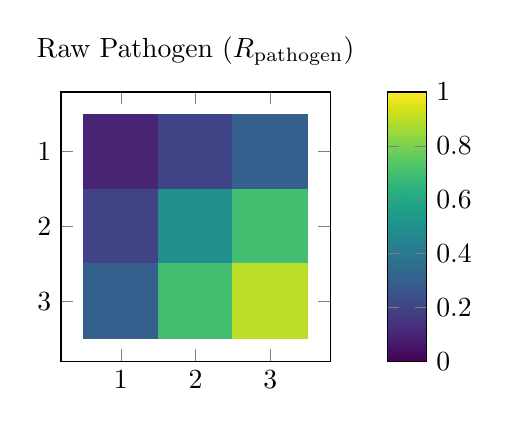
\begin{tikzpicture}
\begin{axis}[
    title={Raw Pathogen ($R_{\mathrm{pathogen}}$)},
    width=5.4cm,height=5.0cm,
    axis equal image,
    xtick={1,2,3}, ytick={1,2,3}, y dir=reverse,
    colorbar, point meta min=0, point meta max=1, colormap/viridis,
]
\addplot[matrix plot*, mesh/cols=3, point meta=explicit] table [meta=C] {
x y C
1 1 0.10
2 1 0.20
3 1 0.30
1 2 0.20
2 2 0.50
3 2 0.70
1 3 0.30
2 3 0.70
3 3 0.90
};
\end{axis}
\end{tikzpicture}
\end{subfigure}
\hfill
\begin{subfigure}{0.45\textwidth}
\centering
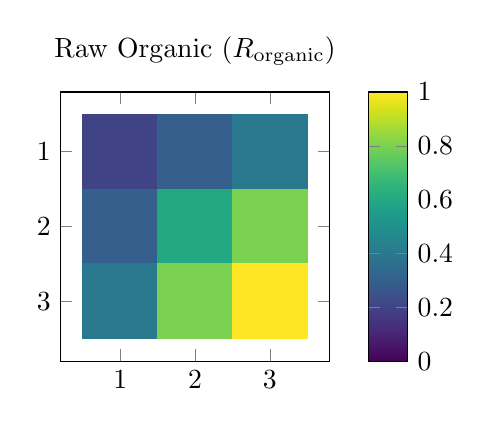
\begin{tikzpicture}
\begin{axis}[
    title={Raw Organic ($R_{\mathrm{organic}}$)},
    width=5.4cm,height=5.0cm,
    axis equal image,
    xtick={1,2,3}, ytick={1,2,3}, y dir=reverse,
    colorbar, point meta min=0, point meta max=1, colormap/viridis,
]
\addplot[matrix plot*, mesh/cols=3, point meta=explicit] table [meta=C] {
x y C
1 1 0.20
2 1 0.30
3 1 0.40
1 2 0.30
2 2 0.60
3 2 0.80
1 3 0.40
2 3 0.80
3 3 1.00
};
\end{axis}
\end{tikzpicture}
\end{subfigure}
\caption{Input raw environmental stress fields.}
\end{figure}

A central feature of the framework is its support for multiple species or target groups (e.g., humans, avian species, aquatic organisms). We denote a specific target group with the superscript $(q)$. Because organisms interact with their environment differently, raw variables are filtered into \textit{effective exposure} $\bm{e}^{(q)}$ via contact, habit, or use multipliers $h_j^{(q)}$:

\begin{equation}
    e_{j, g, m}^{(q)} = h_{j}^{(q)} R_{j, g, m}
\end{equation}

For a fully aquatic species, contact is continuous ($h_j \approx 1.0$). For humans, contact is filtered by drinking water infrastructure, sanitation, and behavioral avoidance ($h_j < 1.0$). 

\section{Phase 2: Mode of Action to DEB Axes Mapping}

Rather than mapping raw exposure directly to organism health, the pipeline processes effective exposure through two intermediate biological layers. 

First, the effective exposure vector is mapped to intermediate \textbf{Modes of Action} $\bm{m}^{(q)}$ (e.g., thermal stress, oxygen depletion, direct toxicity, immune load). This mapping utilizes a linear weight matrix $U^{(q)}$ and a pairwise interaction matrix $\Gamma^{(r,q)}$:

\begin{equation}
 m_{r, g, m}^{(q)} = \sum_{j} U_{rj}^{(q)} e_{j, g, m}^{(q)} + \sum_{j<k} \Gamma_{jk}^{(r,q)} e_{j,g,m}^{(q)} e_{k,g,m}^{(q)}
\end{equation}

Next, these MoA values are mapped to the four core \textbf{DEB physiological axes} $\bm{s}^{(q)}$: Assimilation ($s_A$), Maintenance ($s_M$), Growth ($s_G$), and Reproduction ($s_R$). This step uses a secondary weight matrix $W^{(q)}$ and interactions $\tilde{\Gamma}^{(a,q)}$:

\begin{equation}
 s_{a,g,m}^{(q)} = \sum_{r} W_{ar}^{(q)} m_{r,g,m}^{(q)} + \sum_{r<k} \tilde{\Gamma}_{rk}^{(a,q)} m_{r,g,m}^{(q)} m_{k,g,m}^{(q)}
\end{equation}

By separating MoA from DEB axes, the model easily adapts to different taxa. For instance, hypoxia (an MoA) might heavily penalize assimilation ($s_A$) in fish, but have zero effect on a terrestrial bird. The resulting matrices represent the target group's physiological cost field.

\begin{figure}[H]
\centering
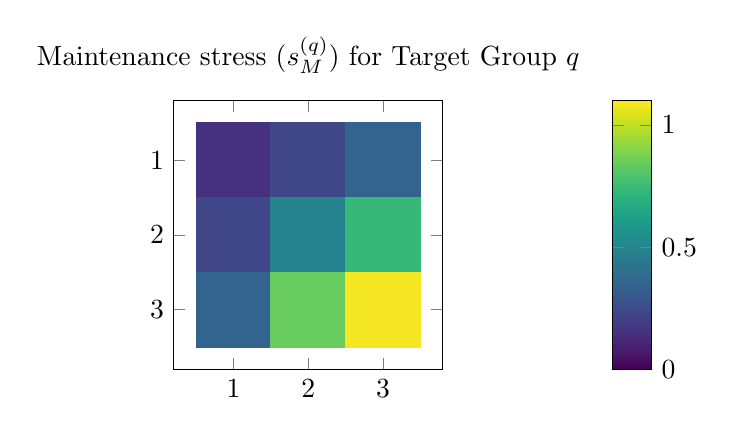
\begin{tikzpicture}
\begin{axis}[
    title={Maintenance stress ($s_M^{(q)}$) for Target Group $q$},
    width=5.4cm,height=5.0cm,
    axis equal image,
    xtick={1,2,3}, ytick={1,2,3}, y dir=reverse,
    colorbar, point meta min=0, point meta max=1.1, colormap/viridis,
]
\addplot[matrix plot*, mesh/cols=3, point meta=explicit] table [meta=C] {
x y C
1 1 0.155
2 1 0.235
3 1 0.350
1 2 0.235
2 2 0.490
3 2 0.735
1 3 0.350
2 3 0.845
3 3 1.085
};
\end{axis}
\end{tikzpicture}
\caption{The calculated physiological maintenance cost raster for species $(q)$, accounting for species-specific exposure filters and MoA mappings.}
\end{figure}

\section{Phase 3: Adaptive Margin and Restoring Force}

The aggregate physiological burden depletes the baseline adaptive capacity ($A_0^{(q)}$) of the species. The scalar \textbf{Adaptive Margin} ($A$) incorporates the DEB axes via sensitivity weights $\bm{\alpha}^{(q)}$. An optional dynamic condition/reserve buffer $Z_{g,m}^{(q)}$ can also be integrated to account for historical depletion or buffering:

\begin{equation}
A_{g,m}^{(q)} = A_0^{(q)} + \omega_Z^{(q)} Z_{g,m}^{(q)} - \sum_{a \in \{A,M,G,R\}} \alpha_a^{(q)} s_{a,g,m}^{(q)}
\end{equation}

The adaptive margin directly determines the \textbf{Restoring Force} ($\lambda^{(q)}$), representing the organism's exponential recovery rate following a perturbation. This is modeled via a bounded Michaelis-Menten formulation:

\begin{equation}
\lambda_{g,m}^{(q)} = \lambda_{\min}^{(q)} + \left(\lambda_{\max}^{(q)} - \lambda_{\min}^{(q)}\right) \frac{\left[A_{g,m}^{(q)}\right]_+}{K_A^{(q)} + \left[A_{g,m}^{(q)}\right]_+}, \qquad \text{where } [A]_+=\max(A,0)
\end{equation}

\begin{figure}[H]
\centering
\begin{subfigure}{0.45\textwidth}
\centering
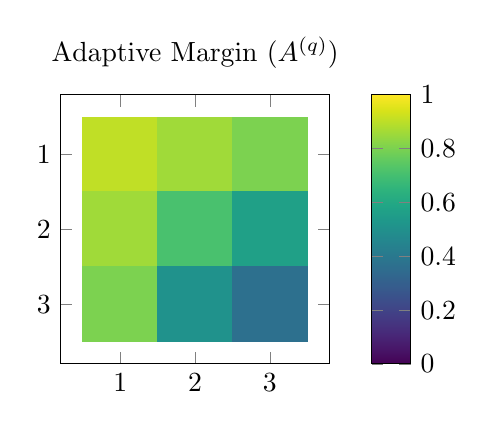
\begin{tikzpicture}
\begin{axis}[title={Adaptive Margin ($A^{(q)}$)},width=5.4cm,height=5.0cm,axis equal image,xtick={1,2,3},ytick={1,2,3},y dir=reverse,colorbar,point meta min=0,point meta max=1,colormap/viridis]
\addplot[matrix plot*, mesh/cols=3, point meta=explicit] table [meta=C] {
x y C
1 1 0.907
2 1 0.859
3 1 0.803
1 2 0.859
2 2 0.711
3 2 0.568
1 3 0.803
2 3 0.509
3 3 0.366
};
\end{axis}
\end{tikzpicture}
\end{subfigure}
\hfill
\begin{subfigure}{0.45\textwidth}
\centering
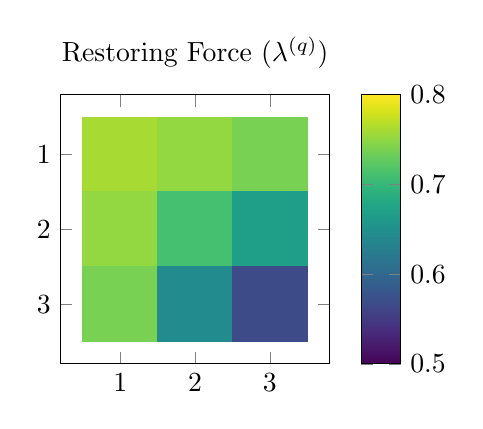
\begin{tikzpicture}
\begin{axis}[title={Restoring Force ($\lambda^{(q)}$)},width=5.4cm,height=5.0cm,axis equal image,xtick={1,2,3},ytick={1,2,3},y dir=reverse,colorbar,point meta min=0.5,point meta max=0.8,colormap/viridis]
\addplot[matrix plot*, mesh/cols=3, point meta=explicit] table [meta=C] {
x y C
1 1 0.761
2 1 0.752
3 1 0.739
1 2 0.752
2 2 0.711
3 2 0.669
1 3 0.739
2 3 0.644
3 3 0.568
};
\end{axis}
\end{tikzpicture}
\end{subfigure}
\caption{Higher physiological costs deplete the adaptive margin, thereby weakening the target group's restoring force.}
\end{figure}

\section{Phase 4: Deriving the Amplification Factor}

Reduced restoring force amplifies the impact of short-term acute perturbations. Let an identical standardized event impose a physiological cost $C_{\mathrm{event}}(t)$. The organism's displacement $y(t)$ from homeostasis is governed by:

\begin{equation}
\frac{dy}{dt} = -\lambda_{g,m}^{(q)}y + q_c C_{\mathrm{event}}(t), \qquad y(0)=0
\end{equation}

The analytical solution for the displacement trajectory is:

\begin{equation}
 y_{g,m}(t) = q_c \int_0^t e^{-\lambda_{g,m}^{(q)}(t-u)}C_{\mathrm{event}}(u)\,du
\end{equation}

We define the total \textbf{Response Burden} as the Area Under the Curve (AUC) of the displacement:

\begin{equation}
\text{AUC}_y(g,m) = \int_0^\infty y_{g,m}(t)\,dt = q_c \int_0^\infty \left[ \int_0^t e^{-\lambda_{g,m}^{(q)}(t-u)}C_{\mathrm{event}}(u)\,du \right] dt
\end{equation}

Applying Fubini's Theorem to reverse the order of integration ($0 \le u \le t < \infty \implies u \le t < \infty$ and $0 \le u < \infty$):

\begin{equation}
\text{AUC}_y(g,m) = q_c \int_0^\infty C_{\mathrm{event}}(u) \left[ \int_u^\infty e^{-\lambda_{g,m}^{(q)}(t-u)}\,dt \right] du
\end{equation}

Evaluating the inner integral by substituting $r = t - u$:

\begin{equation}
\int_u^\infty e^{-\lambda_{g,m}^{(q)}(t-u)}\,dt = \int_0^\infty e^{-\lambda_{g,m}^{(q)}r}\,dr = \frac{1}{\lambda_{g,m}^{(q)}}
\end{equation}

Thus, the total response burden simplifies to:

\begin{equation}
\text{AUC}_y(g,m) = \frac{q_c}{\lambda_{g,m}^{(q)}} \int_0^\infty C_{\mathrm{event}}(u)\,du = \frac{q_c}{\lambda_{g,m}^{(q)}} \text{AUC}_C
\end{equation}

The integral of the event cost ($\text{AUC}_C$) is identical regardless of the background state. To standardize vulnerability, we compute the ratio of the response burden in a stressed grid cell to the response burden under a pristine baseline condition ($A = A_0^{(q)} \implies \lambda_0^{(q)}$):

\begin{equation}
\frac{\text{AUC}_y(g,m)}{\text{AUC}_y(0)} = \frac{\frac{q_c}{\lambda_{g,m}^{(q)}} \text{AUC}_C}{\frac{q_c}{\lambda_0^{(q)}} \text{AUC}_C} = \frac{\lambda_0^{(q)}}{\lambda_{g,m}^{(q)}}
\end{equation}

This confirms that the \textbf{Amplification Factor ($\mathcal{F}^{(q)}$)} is strictly defined by the ratio of the restoring forces:

\begin{equation}
\boxed{ \mathcal{F}_{g,m}^{(q)} = \frac{\lambda^{(q)}(A_0)}{\lambda^{(q)}(A_{\mathrm{DEB},g,m})} }
\end{equation}

\begin{figure}[H]
\centering
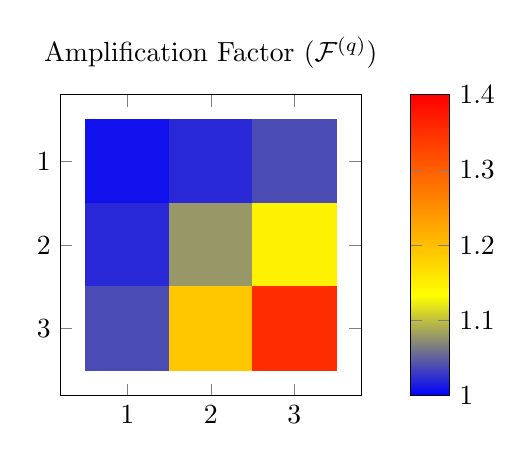
\begin{tikzpicture}
\begin{axis}[
    title={Amplification Factor ($\mathcal{F}^{(q)}$)},
    width=6.0cm,height=5.4cm,
    axis equal image,
    xtick={1,2,3}, ytick={1,2,3}, y dir=reverse,
    colorbar, point meta min=1, point meta max=1.4, colormap/hot,
]
\addplot[matrix plot*, mesh/cols=3, point meta=explicit] table [meta=C] {
x y C
1 1 1.009
2 1 1.021
3 1 1.039
1 2 1.021
2 2 1.079
3 2 1.147
1 3 1.039
2 3 1.192
3 3 1.353
};
\end{axis}
\end{tikzpicture}
\caption{The final spatial result. Background stress conditions local vulnerability, magnifying the impact of future perturbations.}
\end{figure}

\end{document}
